\chapter{Implementation}
The chapter will explain how the different software are connected and what information is sent between them. All the configuration and start up commands can be found in the appendix.
\section{Software implementation}
The software implementation consist mainly of rtklib and dune. Piksi is also used in the experiment, however it's rtklib and the Dune task RTKGPS that will be discussed thoroughly.
\subsection{Rtklib}
Rtklib is sepperated into the base station and the rover. The base station implementation runs the app str2str were it communicate with the ublox over a uart cable, and start up a tcp server.

The rover uses the rtkrcv app from rtklib to estimate the position of the rover. Rtkrcv connect itself as a tcp client to the tcp server that str2str create. Rtkrcv is configured in a moving baseline configuration to simulate the behavior that is expected during a landing on a ship. (Referer her til teori kap om rtklib)

Rtkrcv output the solution data over a virtual uart connection that is created by a program called socat. The output structure is given i (se rtklib com kap)
\subsection{Rtkgps}
Rtkgps is a task in Dune that takes the output from rtklib and create a rtkfix imc message that is dispatch into the Dune/Neptus network. Rtkgps consists of two parts. One reads the message from the virtual uart, and the other create and dispatch the rtkfix imc message.

\subsection{Neptus}
Neptus is used as interface for the human operator, and for after mission reviews. In this thesis it's only used for after mission reviews, however it has the cabillity to give a landing command to the rover (henvis her til frølich)
PLASSERES I APPENDIX
\subsubsection{str2str configuration}
The system has to instances of rtklib. The base station uses the str2str and the x8 uses rtkrcv. str2str is configured to receive raw data from the ublox at a frequency of 10 Hz. The connection between str2str and the GNSS receiver is a uart cable that is configured with a baudrate at 115200. The program starts a tcp serve were rtkrcv becommes a client.

Very short about how Glued is used: Start up, 

About rtklib: What does rtklib do in the system, were do it run, what instances is used, how do it connect to dune, what is the output message

About dune: What task are used to communicate with rtklib, how do they communicate, what is the output of the given task

About Neptus: What do neptus do, how is it used in the system, how will it be used in a automatic landing senario.

About Ardupilot: Very short on what Ardupilot do in the system 



All in one section unless something need more space.
Write here how rtklib is configured and how the system is connected
Write here how Dune receive data from rtklib and what task is used. Include also what imc message is involeved in the task
Write here how neptus is configured for the test, and how it is used
How Glued is configured to run rtklib and Dune
\section{Hardware implementation}
The embedded computer uses GLUED as its operating system, and on it runs both Dune and rtklib. The Piksi and Ublox is connected to the BeagleBone over uart cables.

TRENGER SYSTEM FIGUR SOM VISER HVORDAN UAV ER FORBUNDET MED BASE
The two \gls{rtk-gps} system is connected to a antenna splitter , figure \ref{figure:AntennaSplitter}, such that both system receive the same \gls{gnss} signals.

\begin{figure}[H]
	\centering
		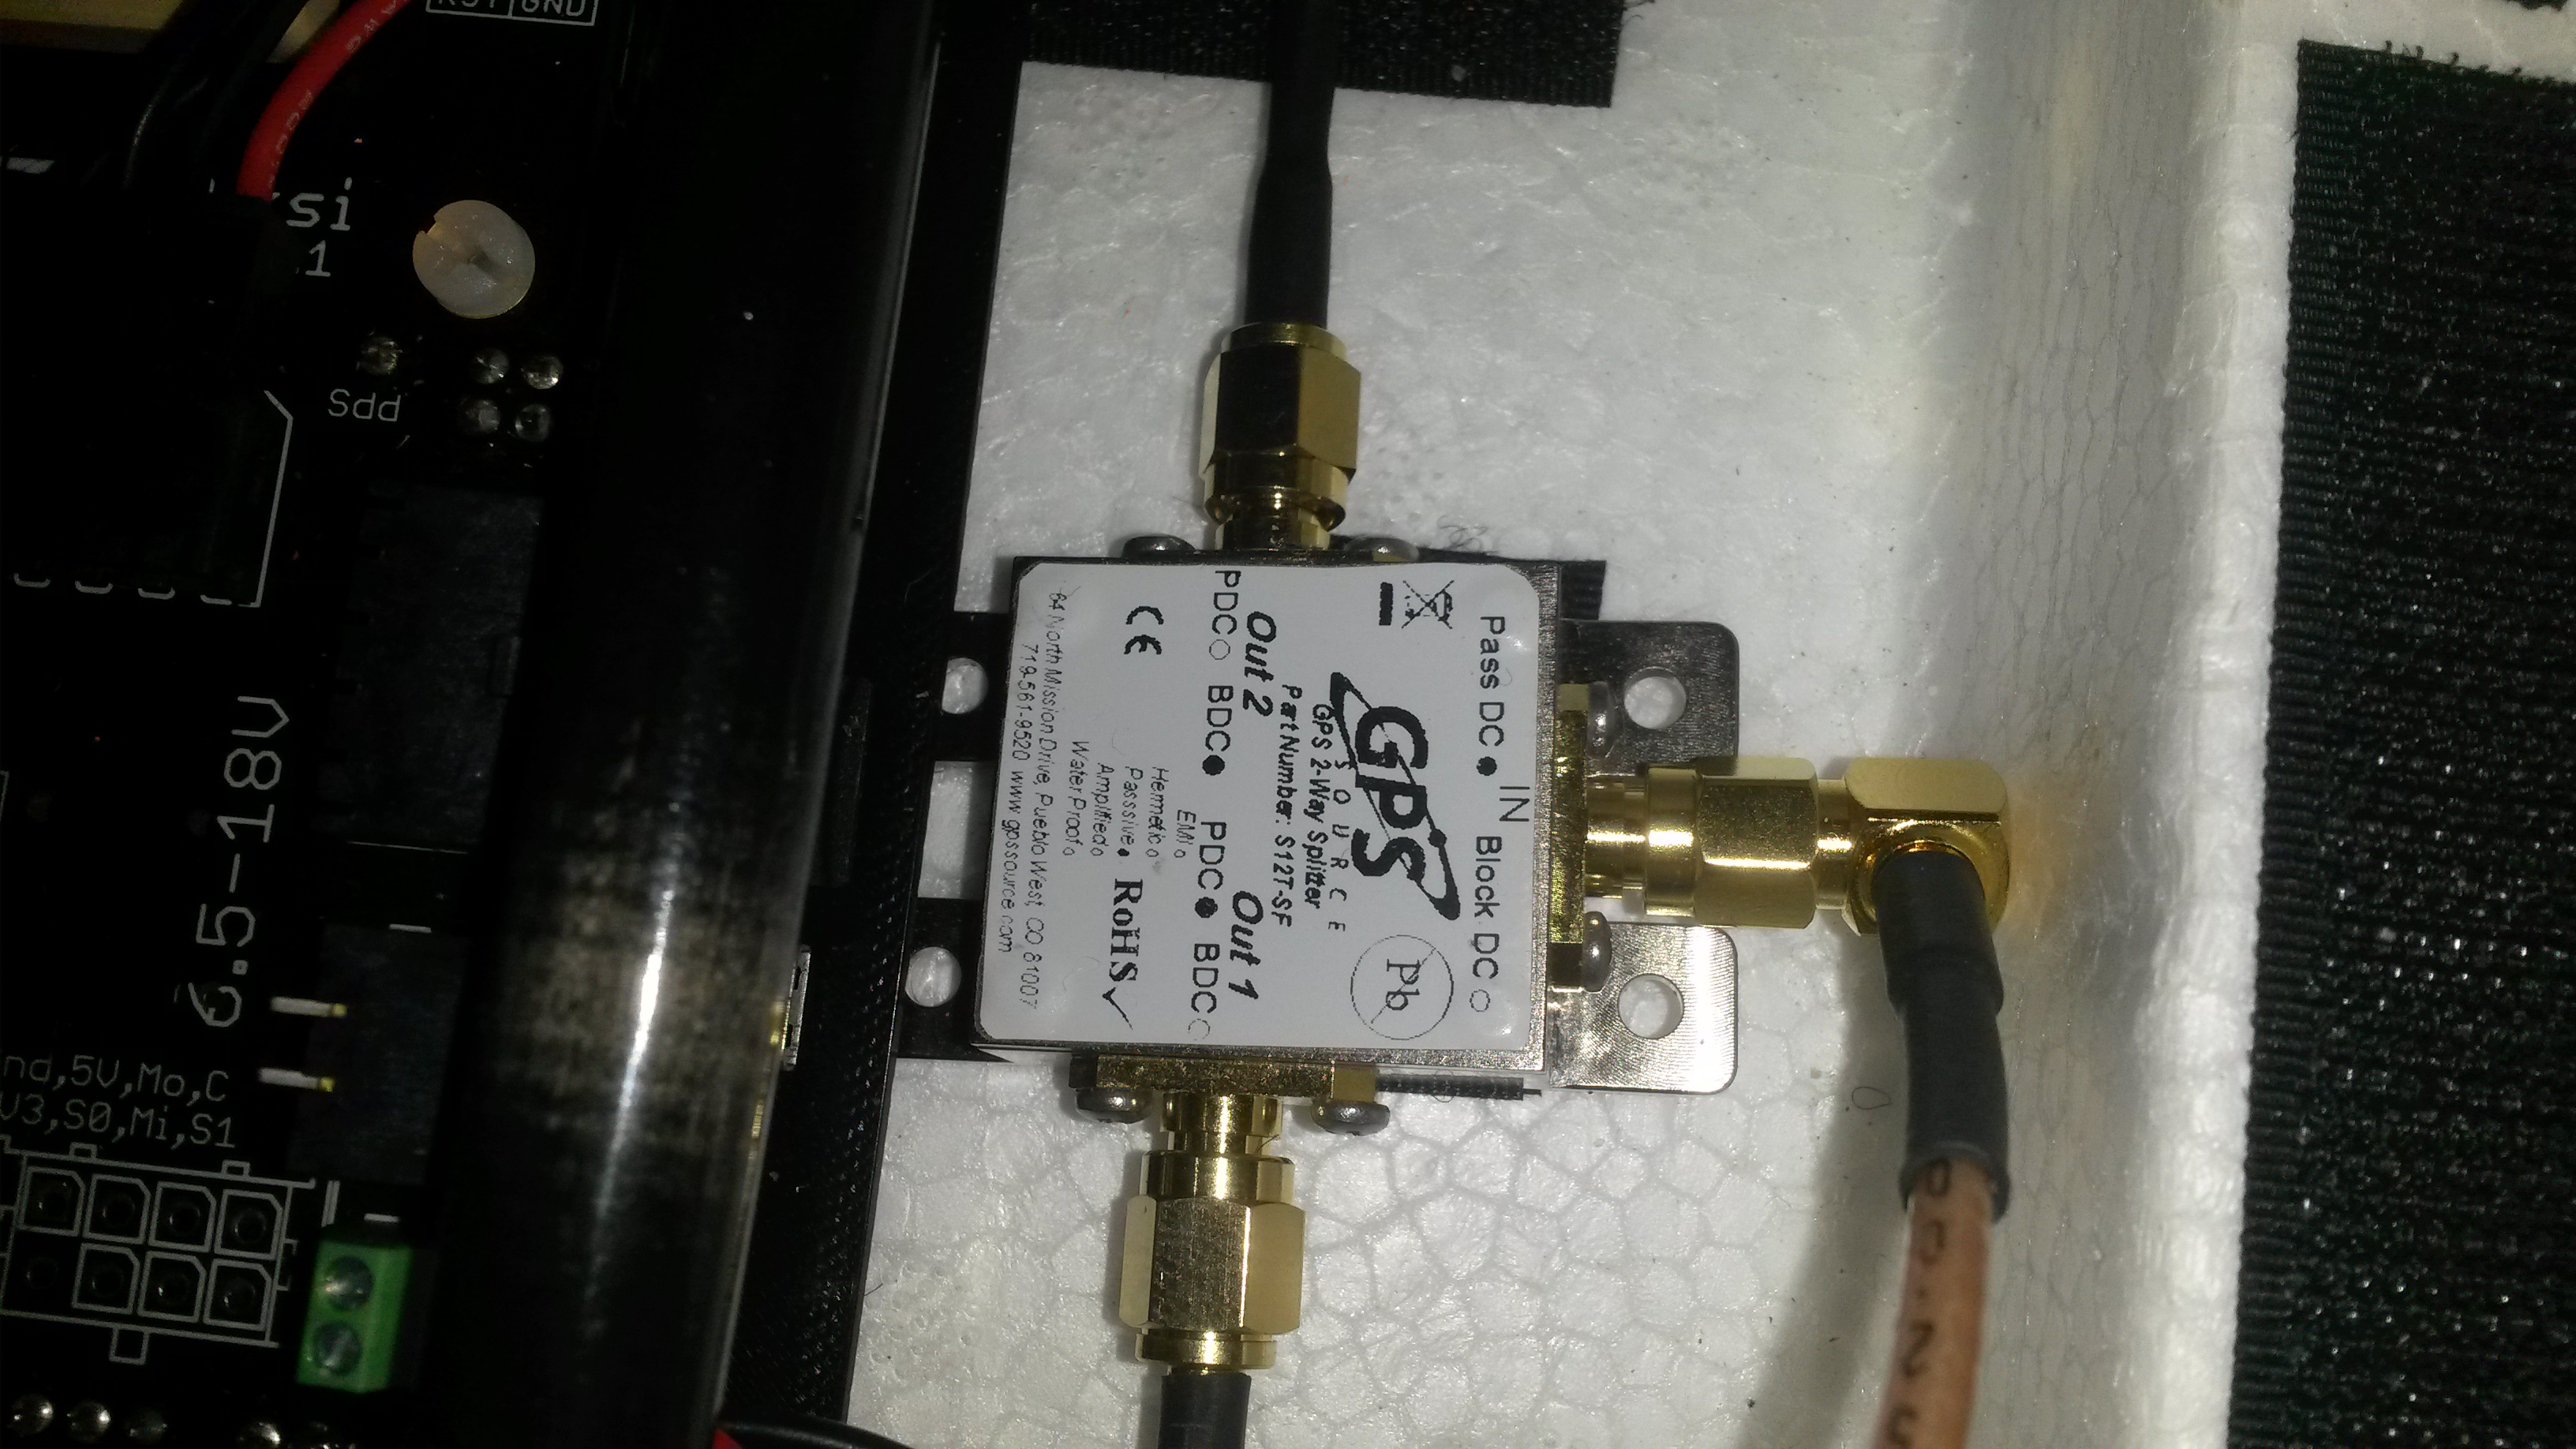
\includegraphics[width=0.7\textwidth]{figs/066.jpg}
		\caption{Antenna splitter}
		\label{figure:AntennaSplitter}
\end{figure}

This section contain how all the physical components are connected at both the rover and the base station. Include also how everything was prepared.

About Beaglebone: What runs on the beaglebone, connections, devices, what is it place in the system

About Ublox: Explain the ublox from a system perspective, how it's connected

Pixhawk: What do it do in the system:

Piksi: Same as ublox

The X8: How do it fit in the system

The base station: Same as x8

Antennas: 

Wifi router

